\documentclass[10pt, a4paper]{article}

\usepackage[utf8]{inputenc}
\usepackage{algorithm}
\usepackage{algorithmic}
\usepackage{amsfonts}
\usepackage[margin=2.5cm]{geometry}
\usepackage{amsmath}
\usepackage{color}
\usepackage{graphicx}
\newcommand{\my}[1]{{\color{blue} #1 }}
\setlength{\parindent}{0pt} 
\floatname{algorithm}{Procedure}
\renewcommand{\algorithmicrequire}{\textbf{Input:}}
\renewcommand{\algorithmicensure}{\textbf{Output:}}
 
\title{Comparing the Jacobi Method and LLL lattice reduction algorithms for cryptographic applications}
\date{Fall 2014}
\author{Frederic Jacobs\\ EPFL Bachelor Semester Project\\ frederic.jacobs@epfl.ch}

\renewcommand{\vec}[1]{\mathbf{#1}}

\begin{document}

\maketitle

\section{Introduction}
\subsection{Results and Contributions}

\my{We show the following main results:
\begin{itemize}
\item An analysis of running times depending on factors
\item paper: \cite{originalJacobiMethodLatticeBasisReduction}
\end{itemize}
}
\subsection{Related Work}

\section{Preliminaries}

In this section, we briefly cover the basics of lattices and lattice reduction required in the scope of this report.

\subsection{Euclidean norm}

The Euclidean norm in $\mathbb{R}^n$ is a mapping from $\mathbb{R}^n \to \mathbb{R}$ that assigns the length to any vector of the space.

The mapping is defined for any vector $\vec{b}$ of $\mathbb{R}^n$ with coordinates $b_i$ as follows: 

\[
\|\mathbf{b}\| = \sqrt{b_1^2 + b_2^2 + ... + b_n^2} 
\] 

which results from the Pythagorean theorem.

\subsection{Lattice, also called Euclidean lattice}

Informally, a lattice can be defined as the infinite set of intersection points of an infinite regular grid.

This can be translated into a more formal definition~\cite{SchnorrStanfordNotes}.\newline 
Let $\vec{b_1}, \vec{b_2}, ... \vec{b_n} \in \mathbb{R}^m$ be linearly independent vectors for $n\leq m$. We call the additive subgroup

\[
L(\vec{b_1}, \vec{b_2},..., \vec{b_n}):= \displaystyle\sum_{i=1}^{n} \vec{b_i} \mathbb{Z}
\] of $\mathbb{R}^m$, a lattice with basis $b_1,b_2,...,b_n$.
A lattice that has $\vec{b_1},\vec{b_2},...,\vec{b_n}$ as basis vectors will be noted in matrix form as $B$ where each vector $\vec{b_i}$ is a column of the matrix.
The \emph{dimension of the lattice} is $dim(L) := rank(L) := n$.

A lattice $L \subseteq \mathbb{R}^m$ is \emph{full dimensional} when $rank(L)=m$. We will work exclusively with full dimensional lattices. In other words, this means that we will work on matrices with $m=n$ linearly independent vectors.

\subsubsection{Equivalent bases}

As this article focuses on lattice basis reduction, it is important to define the equivalence of two bases. Two bases $B_1 , B_2$ are equivalent iff $B_2 = B_1 U$ for a unimodular matrix $U$.

A \emph{unimodular matrix} $U$ is a square integer matrix such that $det(U) = \pm 1$. The right multiplication of a matrix $B$ with a unimodular matrix $U$ yields $B'$ by performing a combination of the following column operations:
\begin{itemize}
\item Swap two columns
\item Negate the elements of a column
\item Addition of an integer multiple of one column to another
\end{itemize}

A lattice can be described by infinitely many equivalent bases. The dimension, the length of a shortest vector and the volume, as described next, stay invariant under change of basis.
\subsubsection{Volume}

The volume of a lattice, also known as the determinant of the lattice, is defined as:
\[
\text{vol} \,L = \sqrt{\det(B^T B)}
\] where $B$ is a matrix of the lattice's basis vectors.


The determinant of an unimodular matrix being $\pm 1$, the determinant is an invariant under change of basis. Therefore the volume of a lattice is an invariant under change of basis.

Since we will be studying full dimensional lattices, the number of basis vectors will be equal to the dimension of the lattice and hence, the volume of the lattice can be computed by taking the absolute value of the determinant of the basis matrix.

For full dimensional lattices, the volume can be computed:
\[
\text{vol} \,L_{\text{full}} = |\det B|
\] where $B$ is a matrix of the linearly independent lattice's basis vectors.


\subsubsection{Minkowski's Convex Body Theorem}

Minkowski's Convex Body Theorem tells us that for a full-rank lattice $L$ of $\mathbb{R}^n$. Let $C$ be a measurable subset of $\mathbb{R}^n$, convex, symmetric with respect to 0, and of measure $> 2^n \text{vol}(L)$. Then $C$ contains at least a nonzero point of the lattice $L$.

A corollary of Minkowski's theorem tells us that there exists for any $n$-dimensional full-rank lattice $L$ a nonzero vector $x$ such that

\[
\lambda_1(L) \leq \sqrt{n} (\det L)^{1/n}
\]

This gives us an upper-bound on the size of a shortest vector in a lattice.

\subsubsection{Hermite Normal Form}

The \emph{Hermite Normal Form} representation of a basis matrix $B$, abbreviated \emph{HNF (B)}, is unique. It is the analogue of the reduced echelon form for integer matrices.

A full-rank matrix $[a_{ij}] \in M_{n,n} (\mathbb{R})$ is in HNF when\cite{SchnorrStanfordNotes} :
\begin{enumerate}
\item $a_{ij} = 0$ for $j > i$, i.e. $A$ is lower triangular. 
\item $a_{ii} > 0$ for $i=1,2,...,n$
\item $0 \leq a_{ij} < a_{ii}$ for $j < i$
\end{enumerate}

\subsection{Special Lattices}

\subsubsection{Random Lattice}

We say that a lattice is a random lattice $L$ of prime volume $P$ if under HNF form its basis matrix $B$ has the following properties:

\begin{itemize}
\item the diagonal has 1 for all it's entries except one position that is set to a prime number $P$. Hence, the $\det(B)$ is prime.
\item All column entries of the matrix under the position that is set to $P$ are smaller than $P$ in absolute value.
\end{itemize}

Without loss of generality, we hence restrict tests to random lattices of volume $P$ whose basis in HNF form is as follows:
$$\begin{array}{ccccc}
P & \vec{a_2} &  & \\
\vec{a_2} & 1&   & \\ 
\dots & &  & \\ 
\vec{a_{m}} & & &1 
\end{array}$$
where $a_i \in \mathbb{Z}/ P\mathbb{Z}$.

\subsubsection{Almost Orthogonal Lattice Bases}

We define a \emph{almost orthogonal lattice basis} $M$ of dimension $n$ and of bit length $k$ as a $n \times n$ square matrix whose entries are $k$-bits picked at random. These lattices are frequently used for signal processing applications~\cite{originalJacobiMethodLatticeBasisReduction}.

\subsection{Lattice Reduction}

Lattice reduction is the process of finding nearly orthogonal vectors from an integer lattice basis. Giving an exact definition of "nearly orthogonal vectors" is tricky and each reduction algorithm is likely to give it's own definition of what it means for a basis to be reduced.

\subsection{Quality of a reduction}

In this section, we will discuss two lattice reduction quality indicators that we will use to compare the result of reduction algorithms.

\subsubsection{Orthogonality defect of a basis}
\label{sec:orthogonalityDefect}
The \emph{orthogonality defect} of a basis $\vec{b_1},\vec{b_2},...,\vec{b_n}$ of a lattice $L$ is defined by:
\[
    \text{OrthDefect}(L) :=  \sqrt[n]{\frac{\displaystyle\prod^{n}_{i=1} \|\vec{b_i}\| }{\det(L)}}
\]

The orthogonality defect is a quality indicator that we will use to compare the reduction of \emph{the set of basis vectors}. The orthogonality defect can be interpreted geometrically as the product of the basis vector lengths divided by the volume of the lattice. As the basis vectors are getting increasingly orthogonal during a reduction, the nominator will become smaller. The lower bound of the orthogonality defect is $\text{OrthDefect} \ge 1$. If $\text{OrthDefect} = 1$, the basis is completely orthogonal.

\subsubsection{Hermite factor of a basis}
\label{sec:hermiteFactor}
The \emph{Hermite Factor} of basis vectors $\vec{b_1}, \vec{b_2},...,\vec{b_n}$ of a lattice $L$ is defined by

\[
    \text{HF}(L) := \frac{\|\vec{b_1}\|}{\sqrt[n]{\det(L)}}
\]

The Hermite Factor is a quality indicator that we will use to compare the reduction to a \emph{shortest vector}.

\subsection{Lattice Hard Problems}

Lattices have a few known hard problems that can be used for asymmetric cryptography. We will only cover the most famous one, the Shortest Vector Problem.

\subsubsection{Shortest Vector Problem (SVP)}

Given a basis of a $n$-rank integral lattice $L$, find $\vec{u} \in L$ such that $\|\vec{u}\| = \lambda_1 (L)$

In other words, we are looking for the shortest vector of the lattice. Finding exactly the shortest vector of a lattice is known to be NP-hard under randomized reductions\cite{Ajtai:1998:SVP} but the complexity of the deterministic reduction remains open.

\subsection{Gram-Schmidt orthogonalization process}
The \emph{Gram-Schmidt orthogonalization (\emph GSO) process} is a method for orthonormalising a set of vectors. Two vectors are orthonormal if they are both orthogonal and unit vectors. 

The GSO process  can be defined recursively:
\[
\begin{cases}
\vec{b_1}^{\star} = \vec{b_i}  \\
\vec{b_i}^{\star} = \displaystyle\sum^{i-1}_{j=1} \mu_{i,j} \vec{b_j^\star}
\end{cases}
\]
where $\mu_{ij} = ..$. Is the set of vectors $b_i^*$ a basis or not? In which case yes?

\section{The LLL Algorithm}

The LLL algorithm~\cite{lllpaper} was the first polynomial-time reduction algorithm to be introduced outputting a nearly orthogonal basis. LLL and BKZ 2.0 are the two reduction algorithms that are used in practice. LLL is used in a first step and BKZ, with a suitable blocksize, is then used in a second step to reduce the basis further if needed.

\subsection{$\delta$-LLL Reduced}
We say that a basis is $\delta$-LLL reduced if:
\begin{itemize}
\item $| \mu_{i,j}| \leq \frac{1}{2} \text{, } \forall i > j$
\item Lovász's condition: $\forall (\vec{b_i, b_{i+1}})$, we have $(\delta - \mu^2_{i+1,i}) \|\vec{b}^{\star}_{i}\|^2 \leq \| \vec{b}^{\star}_{i+1} \|^2$
\end{itemize}

The first condition guarantees the length reduction of the ordered basis.
The Lovász conditions assures us that although the Gram-Schmidt vectors can get shorter and shorter, their length in a sorted basis cannot decrease too quickly.

Since the LLL-reduction algorithm returns a $\delta$-LLL reduced basis, we can observe the following properties on the basis:
\begin{itemize}
\item $\| \vec{b_1} \| \leq \alpha^{(n-1)/2} \lambda_1 $
\item $\max_i \| \vec{b_i} \| \leq \alpha^{(n-1)/2} \lambda_n $
\item $\| b_1 \| \leq \alpha^{(n-1)/4} \det B^{1/n}$
\end{itemize} 
where the parameter $\alpha = 1/(\delta - \frac{1}{4})$. Since $\delta$ is bounded by $1/4 < \delta < 1$, parameter $\alpha \geq 4/3$.

\subsection{LLL overview}

The LLL algorithm, like many reduction algorithms, can be broken down into two parts: size-reduction and vector swapping. Size-reduction reduces the vectors from the input basis. After that, the vectors of the basis are checked against the Lovász condition. If a pair of vectors of the basis $(\vec{b_{i}}, \vec{b_{i+1}})$ don't satisfy the condition, we swap them and go back to the size reduction. my{Procedure 1..}

\begin{algorithm}[H]
\caption{Overview of naive-iterative LLL}
\label{lllAlgorithm}
\begin{algorithmic}[1]
\REQUIRE a basis ($\vec{b_1, ..., b_n}$) of a lattice $L$.
\ENSURE $\delta$-LLL reduced basis $(\vec{b_1, ..., b_n})$

\STATE Size-reduce $(\vec{b_1, ..., b_n})$
\IF{there exists an index $j$ which does not satisfy Lovász' condition} \STATE{swap $\vec{b_j}$ and $\vec{b_{j+1}}$, go back to step 1} \ENDIF

\end{algorithmic}
\end{algorithm}

\section{The Jacobi Method}

In 2012, Sanzheng Qiao suggested to use a Jacobi method for lattice basis reduction\cite{originalJacobiMethodLatticeBasisReduction}. The idea of the Jacobi method is to reduce larger dimension lattice bases by using the Lagrange algorithm iteratively.

\subsection{Lagrange-reduced basis}

Lagrange was the first to formalize\cite{lagrangeArithmetique} the notion of reduction for rank-two lattices.

Let $L$ be a rank-two lattice of $\mathbb{R}^n$. A basis $(\vec{b_1}, \vec{b_2})$ of $L$ is said to be Lagrange-reduced if and only if $\|\vec{b_1}\| \leq \|\vec{b_2}\|$ and $| \langle \vec{b_1} \vec{b_2} \rangle | \leq \| \vec{b_1} \|^2 / 2 $. 

\subsection{Lagrange algorithm}
\label{sec:lagrangeAlgorithm}

Lagrange's algorithm solves the lattice reduction problem exactly for lattice bases of dimension 2. It is a variant of Euler's centered algorithm that is used to compute the greatest common divider of two numbers. GCD can be thought to be a one dimension reduction problem. The GCD is the first minimum of the lattice $n \mathbb{Z} + m \mathbb{Z}$ spanned by $n$ and $m$.

\begin{algorithm}[H]
\caption{Lagrange algorithm}
\label{lagrangeAlgorithm}
\begin{algorithmic}[1]
\REQUIRE a basis ($\vec{b_1, b_2}$) of a lattice $L$ of dimension 2.
\ENSURE a Lagrange reduced reduced basis $(\vec{b_1, b_2})$

\IF{$\|\vec{b_1} \| < \| \vec{b_2} \| $} \STATE{swap $\vec{b_1}$ and $\vec{b_2}$} \ENDIF
\REPEAT \STATE{
$q = \lfloor \frac{ \langle \vec{b_1} \vec{b_2} \rangle }{\| \vec{b_2} \|^2} \rceil $\\
$r \leftarrow \vec{b_1} - q \vec{b_2}$\\
$\vec{b_1} \leftarrow \vec{b_2}$\\
$\vec{b_2} \leftarrow r$
} \UNTIL{$\| \vec{b_1} \| \leq \| \vec{b_2} \| $}

\end{algorithmic}
\end{algorithm}
\subsection{The Generic Jacobi Method}
We call \emph{generic Jacobi method} the algorithm that simply applies the Lagrange algorithm to every pair of the basis vectors for an $n$ dimensional lattice. This method was introduced~my{\cite{originalJacobiMethodLatticeBasisReduction}} by Qiao in 2012 claiming experimental results to be considerably faster than LLL.

From the definition of a Lagrange-reduced basis, we can define a Jacobi-reduced basis such as:
\begin{align}
\langle \vec{b_i} \vec{b_j} \rangle &\leq \frac{1}{2} \| \vec{b_i}\|^2 \text{ (for all $1 \leq i < j \leq n$)}.\\
\| \vec{b_i}\| &\leq \|\vec{b_j} \| \text{ (for all $1 \leq i < j \leq n$)}
\end{align}


\begin{algorithm}[H]
\caption{Generic Jacobi Method}
\label{genericJacobiMethod}
\begin{algorithmic}
\REQUIRE a basis matrix ($\vec{b_1,...,b_n}$)
\ENSURE a generic-Jacobi reduced basis ($\vec{b_1,...,b_n}$)

\WHILE{not all pairs ($\vec{b_i,b_j}$) satisfy both generic-Jacobi reduction conditions}
    \FOR{$i = 1$ \TO $n-1$ }
        \FOR{$j = i + 1$ \TO $n$ }
            \STATE {$[\vec{b_i, b_j}]$} = \emph{Lagrange$(\vec{b_i, b_j})$}
        \ENDFOR
    \ENDFOR
\ENDWHILE

\end{algorithmic}
\end{algorithm}

\subsection{A Jacobi Variant}

In this part, we present the Jacobi-variant that was used for running our benchmarking.

\subsubsection{$\omega$-Lagrange-reduced conditions}
An $\omega$ is introduced to 
There are two conditions for a basis to be $\omega$-Lagrange-reduced.

\[
\begin{cases}
\lfloor g_{ij} / g_{ss} \rceil \leq 1, \\
\omega^2 g_{ll} \leq g_{ii} + g_{jj} - 2|g_{ij}|

\end{cases}
\]  where $1/\sqrt{3} \leq \omega < 1$.

\subsubsection{Size-reduction Lagrange}
The size-reduction algorithm is a variant of the Lagrange algorithm that we presented in section \ref{sec:lagrangeAlgorithm}. The reduction is only performed if the $\omega$-Lagrange-reduced conditions are not satisfied. In which case, both the unimodular reduction matrix $Z$ and the Gram matrix $G$ are updated by applying the Lagrange reduction to the longest of the basis vectors at index $i$ or $j$.

\begin{algorithm}[H]
\caption{LagrangeIT}
\label{customLagrangeIT}
\begin{algorithmic}
\REQUIRE The matrices $G, Z$, a pair of indices $(i,j):i<j$ and a parameter $\omega$
\ENSURE  Updated $G, Z$ where one Lagrange iteration was performed on the $i$th and $j$th basis vectors. 

\STATE {$s \leftarrow i$}
\STATE {$l \leftarrow j$}

\IF{$g_{ii} > g_{jj}$}
    \STATE {$s \leftarrow j; l \leftarrow i$}
\ENDIF

\STATE{$q \leftarrow \lfloor \frac {g_{ll}}{g_{ss}} \rceil $}

\IF {Verify both $\omega$-Lagrange-reduced conditions}

\STATE{$\vec{z}_l -= q* \vec{z}_s$}
\STATE{$\vec{g}_l -= q* \vec{g}_s$}

\FOR{every column $k$ of $G$}
\STATE{$g_{lk} = g_{kl} $}
\ENDFOR

\STATE{$g_{ll} -= q* g_{ls} $}
\ENDIF

\end{algorithmic}
\end{algorithm}
\my{Please make sure that there is no mistake above. I will check it later. Syntax}

\subsection{Jacobi-variant algorithm}
This Jacobi-variant performs Lagrange reductions iteratively on the Gram matrix until no more reduction is done. That is when both $\omega$-reduced Lagrange conditions are satisfied. 

\begin{algorithm}[H]
\caption{Jacobi-Variant Reduction}
\label{jacobiVariantReduction}
\begin{algorithmic}
\REQUIRE a basis matrix ($\vec{B = b_1,...,b_n}$) and $\omega$
\ENSURE a reduced basis ($\vec{b_1,...,b_n}$) where each pair of vectors is $\omega$-Lagrange reduced
\STATE{$G = \langle B^T B \rangle$, $Z = I_n$}
\WHILE{LagrangeIT method reduced the basis vectors}
    \FOR{$i = 1$ \TO $n-1$ }
        \FOR{$j = i + 1$ \TO $n$ }
            \STATE {$[G, Z]$} = \emph{LagrangeIT$(G,Z,i,j,\omega)$}
        \ENDFOR
    \ENDFOR
\ENDWHILE

\end{algorithmic}
\end{algorithm}

\section{Experimental Results}

\subsection{Our Implementation}

We implemented this Jacobi algorithm in C++ with the \emph{newNTL} library. The FPLLL implementation was used for LLL reductions.

\subsection{Scope of testing}

Our experimentation focused on the quality of the reduction. The two quality metics we used for comparing the reductions are:

\begin{itemize}
\item the orthogonality defect (See section: \ref{sec:orthogonalityDefect}), gives us an indication about the size of the reduced basis vectors for a given lattice.
\item the Hermite factor (See section: \ref{sec:hermiteFactor}), gives us an indication about the size of the shortest vector of the reduced basis for a given lattice.
\end{itemize}

\subsection{Input bases}
Numerous papers were written about the Jacobi method for lattice reduction by S. Qiao \cite{originalJacobiMethodLatticeBasisReduction}\cite{complexityAnalysisOfJacobiMethod}\cite{enhancedJacobi} but none of the papers are clarifying what bitsize was used for the randomly generated entries of the vectors. The main focus of the authors was the use of lattice reduction for signal processing, more specifically multiinput and multioutput (MIMO), the use of multiple antennas at both the transmitter and receiver to improve communication reliance. MIMO uses smaller dimensions lattices. \cite{enhancedJacobi} and \cite{tian2014hybrid}  are using lattices that are at most 20 and  100 dimensions respectively. These dimensions are inappropriate for cryptographic applications.

In our experiments, we have used a bitsize of around 10 bits entries when generating the almost orthogonal bases.

\subsection{On Almost Orthogonal Basis}

We initially ran our Jacobi reduction variant on almost orthogonal bases to attempt to reproduce Qiao's results.

\begin{figure}[h!]
  \caption{LLL with delta $\delta = 0.99$ and Jacobi with $\omega = 0.6$}
  \centering
    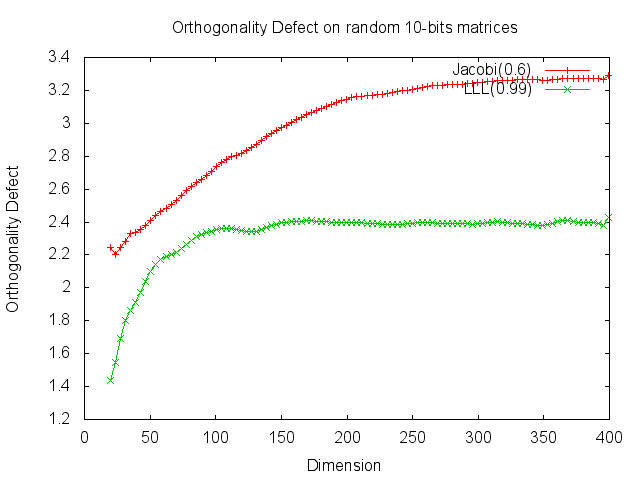
\includegraphics[width=0.5\textwidth]{random-matrix-omega-06defect.png}
\end{figure}

\begin{figure}[h!]
  \caption{LLL with delta $\delta = 0.99$ and Jacobi with $\omega = 0.99$}
  \centering
    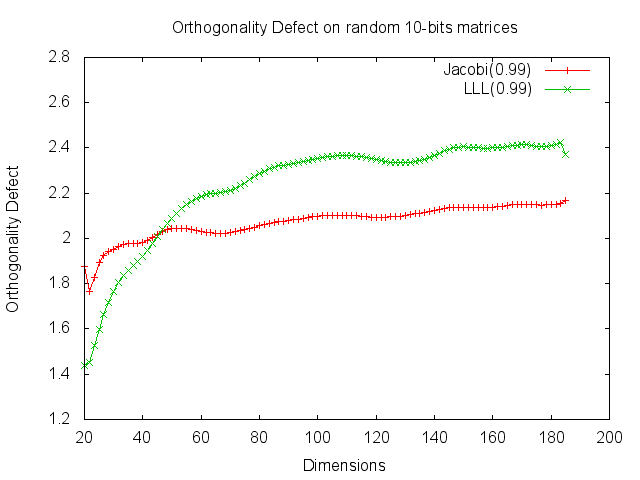
\includegraphics[width=0.5\textwidth]{random-matrix-omega-09defect.png}
\end{figure}

These orthogonality defects are similar to that the authors found in \cite{tian2014hybrid}.

\subsection{Random Lattices}

TODO: 

\subsection{Jacobi after LLL}

We notice that the Jacobi algorithm does reduce the bases further than LLL.

We show two examples of bases that are LLL-reduced but not $\omega > 0.9$ Jacobi reduced.

\begin{enumerate}

\item \[
B = \begin{bmatrix}
  \vec{b_1} \\
  \vec{b_2} \\
  \vec{b_3}
 \end{bmatrix} = \begin{bmatrix}
  0 & 2 & 0 \\
  0 & 1 & 2 \\
  2 & 0 & 0
 \end{bmatrix}
\]


\item \[
B = \begin{bmatrix}
  \vec{b_1} \\
  \vec{b_2} \\
  \vec{b_3}
 \end{bmatrix} = \begin{bmatrix}
  4/3 & 0 & 0 \\
  2/3 & \sqrt{4/3} & 0 \\
  2/3 & \sqrt{4/3}/2 & 1
 \end{bmatrix}
\]

In the first case, LLL will stop while Jacobi does exchange $B-2$ and $b_3$. In the second case the Jacobi Method will find a shortest vector by subtracting $\vec{b_1}-\vec{b_2}$, while LLL won't be able to reduce further.
\end{enumerate}

\subsection{Note on running times}
Although the analysis of the running time was not a metric that was researched in this paper, we did notice that the Jacobi method running time was growing substantially with the dimensions. We were unable to reproduce reduction running times lower than those of LLL as reported by the authors.



\section{Conclusions}

\bibliographystyle{alpha}
\bibliography{references}

\section{Credits}

\end{document}